% !TEX root =  ./main.tex


\subsection{T cell differentiation analysis}\label{sec:datamod2023}

\textcolor{blue}{The paper~\cite{datamod2023-NaCo} (being the full and corrected version of~\cite{datamod2023}, see also Footnote~\ref{correction})} exploits Reaction Systems to analyse T cell differentiation in the immune system, a widely studied biological phenomenon. The starting point for the analysis is a Boolean network model; several of those are available as a \cite{saez2007logical,thakar2010boolean,puniya2018mechanistic}, among which the one in \cite{puniya2018mechanistic} was selected. The model encompasses reactions enabling T cells to manifest various phenotypes in response to environmental stimuli, and describes a realistic regulation system that is involved in many diseases \cite{lafaille1998role,hirahara2016cd4+,meng2016regulatory}.
% it has been investigated under both the viewpoints of causality (effect of environmental conditions) and of reachability (reachable phenotypes). 

The Boolean network model is graphically represented as shown in Fig.~\ref{fig:model-graph}, where the 9 orange nodes represent different environmental stimuli that the T cell can receive; all the other nodes represent so-called \emph{transcription factors} and have an associated Boolean update formula that specifies when they are triggered. 
%The analysis allowed to uncover the genes necessary for the expression of a target transcription factor.
%The analysis of the model allowed to determine which combinations of stimuli lead to each phenotype, and also which proteins inside T cells are involved in each case. 
T cells can manifest four phenotypes, 
%\texttt{Th1}, \texttt{Th2}, \texttt{Th17} and \texttt{iTreg}, 
represented by the four transcription factors \texttt{tbet}, \texttt{gata3}, \texttt{rorgt} and \texttt{foxp3}, respectively.
%The case in which none of the four relevant transcription factors is expressed (i.e., no phenotype is exhibited) is denoted as Th0.
There exists experimental and computational evidence that a T cell can manifest more than one phenotype \cite{luckheeram2012cd4+,puniya2018mechanistic}.

\begin{figure}[t]
	\begin{center}
		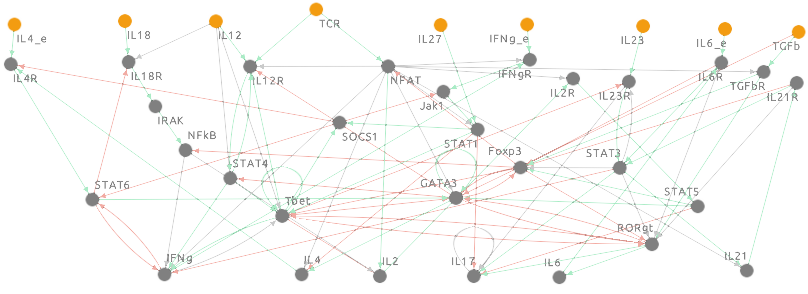
\includegraphics[width=\columnwidth]{figs-datamod2023/Tcell-graph-8set23.png}
	\end{center}
	\caption{Graphical representation of the Boolean network model of T cell differentiation from \cite{puniya2018mechanistic}.}
	\label{fig:model-graph}
\end{figure}

\subparagraph*{Analysis goals.}
The reachability analysis must take into account the different combinations of phenotypes that a T cell can express, called a \emph{target} (hence, $2^4=16$ targets overall).
For example, for the target containing the combination of transcription factors $\{\texttt{tbet},\texttt{gata3}\}$, we must select an attractor that includes at least one state in which $\texttt{tbet}$ is present, at least one state (possibly the same) in which $\texttt{gata3}$ is present, and no state in which either $\texttt{rorgt}$ or $\texttt{foxp3}$ are present. 
The causal analysis aims to collect the combinations of environmental stimuli that are responsible for leading to that target.

\subparagraph*{Features of interest.}
We have selected this case study because it shows the applicability of our method to Boolean networks models, like those available in the public database on the CellCollective platform~\cite{helikar2012cell}. 
For these models, the most relevant viewpoints are often reachability (e.g., \emph{which phenotypes are reachable?}) and causality (\emph{what is the effect of environmental conditions?}) analyses.
Their corresponding RSs always use a special kind of nondeterministic persistent context, where at the beginning of the experiment a subset of external stimuli is chosen and then provided at each subsequent step, inevitably causing the RS to end up in a loop (called an attractor).

\subparagraph*{Experimental set up.}

The translation from Boolean networks to RS consists in turning every update formula into disjunctive normal form. Then, every clause of the disjunction produces a reaction in which (i) reactants are the positive atoms, (ii) inhibitors are the negated atoms and (iii) the updated variable forms a singleton product. 
%
%The RS model of T cell differentiation obtained from the translation of the Boolean model is given in Fig. \ref{fig:RS-reactions}.
%
%\begin{figure}[t]
%\fontsize{7}{0}
%\begin{verbatim}
%react([il4r],[socs1,ifng],[stat6]),         react([tgfb,nfat],[void],[tgfbr]),
%react([tbet],[void],[il12r]),               react([stat4],[gata3],[il2r]),
%react([tcr],[gata3],[il12r]),               react([il12,nfat],[void],[il12r]),
%react([il2r],[void],[stat5]),               react([gata3],[tbet],[gata3]),
%react([stat5],[tgfb,rorgt,foxp3,tbet],[gata3]),
%react([stat6,nfat],[tgfb,rorgt,foxp3,tbet],[gata3]),
%react([stat3],[void],[il23r]),              react([il23,stat3],[tbet],[il23r]), 
%react([tbet],[stat3],[ifng]),               react([nfkb],[void],[ifng]),
%react([stat4,nfkb,nfat],[stat6,stat3],[ifng]),
%react([tgfbr,stat3,il6r],[tbet,gata3,foxp3],[rorgt]),
%react([tgfbr,stat3,il21r],[tbet,gata3,foxp3],[rorgt]),
%react([il21],[void],[il21r]),               react([il18,il12],[stat6],[il18r]),
%react([il6e],[void],[il6r]),                react([il6],[void],[il6r]),
%react([il18r],[void],[irak]),               react([il12r,il12],[gata3],[stat4]),
%react([tbet],[void],[socs1]),               react([stat1],[void],[socs1]),
%react([gata3,nfat],[stat1],[il4]),          react([stat3,nfat],[void],[il21]),
%react([rorgt],[void],[il6]),                react([stat5],[il21r,il6r,gata3],[foxp3]),
%react([stat5],[il21r,stat3,gata3],[foxp3]), react([tgfbr],[il21r,il6r,gata3],[foxp3]),
%react([tgfbr],[il21r,stat3,gata3],[foxp3]), react([tbet],[ifng,il12,rorgt,foxp3],[tbet]),
%react([stat4],[rorgt,foxp3],[tbet]),        react([stat1],[rorgt,foxp3],[tbet]),
%react([il27,nfat],[void],[stat1]),          react([jak1],[void],[stat1]),
%react([il21r],[void],[stat3]),              react([il23r],[void],[stat3]),
%react([il6r],[void],[stat3]),               react([ifngr],[socs1],[jak1]),
%react([il2,nfat],[void],[il2r]),            react([il4e],[void],[il4r]),
%react([il4],[socs1],[il4r]),                react([irak],[foxp3],[nfkb]),
%react([tcr],[foxp3],[nfat]),                react([stat3,il17,il23r],[stat1,stat5],[il17]),
%react([rorgt],[stat1],[il17]),              react([nfat,nfkb],[tbet],[il2]),
%react([ifng,nfat],[void],[ifngr]),          react([ifnge,nfat],[void],[ifngr])
%\end{verbatim}
%\normalsize
%\caption{Reactions of the RS model in BioReSolve syntax.}
%\label{fig:RS-reactions}
%\end{figure}
%
The translation from Boolean network to \BioResolve syntax is done using the directive \verb=main_do(bn2rs)=.
For the readers' convenience, all update formulas and the resulting reactions are reported, respectively, in \Cref{fig:boolean-formulas} and in \Cref{fig:bioresolve:tcell} in the Appendix. 
For example, the update formula for \texttt{IL12R} is
%
\begin{small}
\[
 (\mathtt{IL12} \& \mathtt{NFAT})~|~(\mathtt{STAT4} \& \neg \mathtt{GATA3})~|~ \mathtt{Tbet}~|~(\mathtt{TCR} \& \neg \mathtt{GATA3})
\]
\end{small}
%
which yields the four reactions:\footnote{\label{correction}\textcolor{blue}{The specification analysed in~\cite{datamod2023-NaCo}, on which this paper is based, repairs a minor typo in the original conference version~\cite{datamod2023}. Specifically, the product set of the reaction $\mathtt{({stat4},{gata3},{il12r})}$ was mistakenly written as $\mathtt{il2r}$, omitting the digit $\mathtt{1}$. Unfortunately, since $\mathtt{il2r}$ was also a valid entity, the error was difficult to detect. Though the mistake mildly affected the original results, it turns out that for the analysis reported in this paper there is no difference at all.}}
%
\begin{small}
\[
\begin{array}{c@{{\quad}}c}
\mathtt{(\{il12,nfat\},\emptyset,\{il12r\})}
 & \mathtt{(\{stat4\},\{gata3\},\{il12r\})} \\
\mathtt{(\{tbet\},\emptyset,\{il12r\})}
 & \mathtt{(\{tcr\},\{gata3\},\{il12r\})} \\ 
\end{array} 
\]
\end{small}

The RS context can choose any combination of environmental stimuli that will then persist, i.e., for each possible stimulus $s$ we define the context processes $\mathsf{X}_s \triangleq \{\mathsf{s}\}.\mathsf{X}_s$
%\[
%\begin{array}{rllrll}
%\mathsf{X}_s & \triangleq & \{\mathsf{s}\}.\mathsf{X}'_s + \mathsf{Emp} &\quad
%\mathsf{X}'_s & \triangleq & \{\mathsf{s}\}.\mathsf{X}'_s
%\end{array}
%\]
%
and then take the context $\prod_s (\mathsf{X}_s + \mathsf{Emp})$.
%\[
%\begin{array}{rllrll}
%\mathsf{X1} & \triangleq & \{\mathsf{TGFb}\}.\mathsf{X11} + \mathsf{Emp} &\quad
%\mathsf{X11} & \triangleq & \{\mathsf{TGFb}\}.\mathsf{X11}\\
%\mathsf{X2} & \triangleq & \{\mathsf{IL23}\}.\mathsf{X21} + \mathsf{Emp} &\quad
%\mathsf{X21} & \triangleq & \{\mathsf{IL23}\}.\mathsf{X21}\\
%\mathsf{X3} & \triangleq & \{\mathsf{IL12}\}.\mathsf{X31} + \mathsf{Emp} &\quad
%\mathsf{X31} & \triangleq & \{\mathsf{IL12}\}.\mathsf{X31}\\
%\mathsf{X4} & \triangleq & \{\mathsf{IL18}\}.\mathsf{X41} + \mathsf{Emp} &\quad
%\mathsf{X41} & \triangleq & \{\mathsf{IL18}\}.\mathsf{X41}\\
%\mathsf{X5} & \triangleq & \{\mathsf{IL4e}\}.\mathsf{X51} + \mathsf{Emp} &\quad
%\mathsf{X51} & \triangleq & \{\mathsf{IL4e}\}.\mathsf{X51}\\
%\mathsf{X6} & \triangleq & \{\mathsf{IL27}\}.\mathsf{X61} + \mathsf{Emp} &\quad
%\mathsf{X61} & \triangleq & \{\mathsf{IL27}\}.\mathsf{X61}\\
%\mathsf{X7} & \triangleq & \{\mathsf{IL6e}\}.\mathsf{X71} + \mathsf{Emp} &\quad
%\mathsf{X71} & \triangleq & \{\mathsf{IL6e}\}.\mathsf{X71}\\
%\mathsf{X8} & \triangleq & \{\mathsf{IFNge}\}.\mathsf{X81} + \mathsf{Emp} &\quad
%\mathsf{X81} & \triangleq & \{\mathsf{IFNge}\}.\mathsf{X81}\\
%\mathsf{X9} & \triangleq & \{\mathsf{TCR}\}.\mathsf{X91} + \mathsf{Emp} &\quad
%\mathsf{X91} & \triangleq & \{\mathsf{TCR}\}.\mathsf{X91}\\
%\end{array}
%\]
The resulting LTS has an initial branching into $2^9$ different states, because there are $9$ possible stimuli to be considered. Subsequently, each of the $2^9$ states originates a deterministic computation, leading to some attractors. 

\subparagraph*{Previous approach.}
The paper~\cite{datamod2023-NaCo} presents a toolchain (\BioResolve, SWI-Prolog, Python and Python-to-Prolog binding facilitated by the \verb=swiplserver= Python package) to study the Boolean network model. Roughly, after translating the Boolean network model to RS specifications the whole LTS  is constructed according to any combination of persistent stimuli that can be provided by the context. \BioResolve returns the LTS as a graph in dot format, which is then loaded by a Python script. Then, attractors related with a target of interest are identified by looking for cycles in the LTS, and a slicing algorithm performs some form of causal analysis, to simplify each computation trace by preserving only the relevant causes of those target entities. 
The generation of the LTS is often the bottleneck of the approach, both in terms of time (Prolog performance), but also in terms of space, because \BioResolve can require to allocate a large stack limit size to succeed. 

% 
%Finally, the results of slicing analysis are summarized in Figure \ref{fig:slicing-result}, where it is possibile to see, for each target, which internal genes are \emph{strictly necessary} and which are somehow \emph{relevant} for the expression of the transcription factor of the target. 
%
%Each combination inevitably leads to a looping behaviour (called attractors). Then, the Python script conducts an analysis of the attractors w.r.t. some given \emph{target} entities, and the slicing algorithm performs some form of causal analysis, to simplify each computation trace by preserving only the relevant causes of those  target entities. 

%In Table \ref{tab:context-count} we report the number of different contexts (choices of environmental stimuli) that lead to each target. The table shows only targets that can be reached, and they result to be those in which only one transcription factor is expressed, and those in which Tbet is expressed together with another transcription factor. For each target, the contexts leading to it are summarized in the table by a Boolean formula, while in Figure \ref{fig:input-composition} they are depicted graphically. 
%
%\begin{table}[t]
%	\begin{center}
%		\scriptsize
%		\begin{tabular}{|l|c|l|}
%			\hline
%			{\bf Target} & {\bf Contexts} & {\bf Formula}\\
%			\hline
%			Tbet			&	76 		& (not X11) and (X91) and\\
%			&			& ( ((not X31) and (X61))\\
%			&			& \ \ or ((not X31) and (not X61) and (X71) and (X81))\\
%			&			& \ \ or ((not X31) and (not X51) and (not X61) and (not X71) and (X81))\\
%			&			& \ \ or ((X31) and (X71)) )\\
%			\hline
%			GATA3			&	8		& (not X11) and (not X31) and (X51) and \\
%			&			& (not X61) and (not X81) and (X91) \\
%			\hline
%			Foxp3			&	72		& (not X71) and (not X91) and \\
%			& 			& ( ((X11) and (not X61) and (not X81))\\
%			& 			& \ \ or (X31) )\\
%			\hline
%			RORgt			&	16		& (X11) and (not X31) and (not X61) and (X71) and (X91) \\
%			\hline
%			Tbet,GATA3		&	4		& (not X11) and (not X31) and (X51) and \\ 
%			&			& (not X61) and (not X71) and (X81) and (X91) \\
%			\hline
%			Tbet,Foxp3		&	24		& (X11) and (not X31) and (not X71) and (X91)
%			and 
%			( (X61) or (X81) )  \\
%			\hline
%			Tbet,RORgt		&	48		& (X11) and (X71) and (X91)
%			and ( (X31) or (X61) ) \\
%			\hline
%			%		GATA3,Foxp3		& & \\
%			%		GATA3,Rorgt		& & \\
%			%		Foxp3,Rorgt		& & \\
%			%		Tbet,GATA3,Foxp3	& 0 & $false$\\
%			%		Tbet,GATA3,Rorgt	& & \\
%			%		Tbet,Foxp3,Rorgt	& & \\
%			%		GATA3,Foxp3,Rorgt	& & \\
%			%		Tbet,GATA3,Foxp3,Rorgt	& & \\
%			%		\hline
%			{\bf TOTAL}			& {\bf 248} & \\
%			\hline
%		\end{tabular}
%		\normalsize
%	\end{center}
%	\caption{Summary of contexts leading to each reachable target.}
%	\label{tab:context-count}
%\end{table}
%

%In the end, it is shown that 248 contexts (out of 512) lead to the expression of at least one of the four transcription factors under study, with Tbet, corresponding to phenotype Th1, being expressed in the majority of the cases (152 out of 248), half of the times in combination with another transcription factor.
%% (in 76 cases out of 152). 
%%Also Foxp3 is often expressed (in 96 cases out of 248), while RORgt and GATA3 are less frequent (64 and 12 cases, respectively).
%Moreover, it is observed that:
%\begin{itemize}
%	\item TCR has to be present in order to express any of the phenotypes
%	\item IL23R and IL18R do not contribute to determine any of the phenotypes
%	\item The presence of TGFb mostly discriminates between the expression of either Foxp3/RORgt or tbet/GATA3.
%\end{itemize}


%\begin{figure}[t]
%	\begin{center}
%		\includegraphics[width=12cm]{images/input_composition.png}
%	\end{center}
%	\caption{Graphical representation of the Boolean formula given in Table \ref{tab:context-count} and characterizing contexts leading to each reachable target. Green cells denote that the corresponding environmental stimulus has to be present, red cells denote absences, and white cells denote that the stimulus is irrelevant.}
%	\label{fig:input-composition}
%\end{figure}
%
%
%Fig. \ref{fig:input-composition} allows us to make the following main observations about the role of the environment in the T cell differentiation process:
%\begin{itemize}
%	\item TCR has to be present in order to express any of the phenotypes
%	\item IL23R and IL18R do not contribute to determine any of the phenotypes
%	\item The presence of TGFb mostly discriminates between the expression of either Foxp3/RORgt or tbet/GATA3.
%\end{itemize}
%Moreover, the detailed characterization of the contexts leading to the expression of each phenotype could allow several more specific observations to be done.

%The results of the analysis we conducted partially agree with those of a similar analysis done in \cite{puniya2018mechanistic}. However, there are also some significant differences between the results of the two studies. First of all, in \cite{puniya2018mechanistic} the authors show that it is also possibile to reach configurations in which three or four (i.e., all) phenotypes are expressed. Morevoer, they show that a configuration in which only RORgt is expressed cannot be reached. The Boolean network we started from is exactly the same as the one considered in \cite{puniya2018mechanistic}. The main difference between the two analysis approaches lies in the semantics of the environment: in our case the environment is modelled by a context process that remains the same after the initial non-deterministic choice, while in \cite{puniya2018mechanistic} the analysis is performed by applying a simulation method that allows activity levels and noise to be taken into account for the input species. Hence, the method applied in \cite{puniya2018mechanistic} can lead to a larger range of hypotheses about the modelled system behaviours (such as the possibility for T cell to express more than two phenotypes), while ours is more conservative and consistent with the standard simulation approaches. 

%For each target, slicing analysis is conducted by invoking the \verb=main_do(slice,S)= directive of BioReSolve for each state of each attractor of the target. This is obtained by implementing suitable nested loops in the Python script that, at each iteration, execute BioReSolve through the Python-to-Prolog binding provided by the \verb=swiplserver= package.  
%
%Slicing analysis in BioReSolve requires, in addition to the RS reactions, to provide the specification of a monitor (i.e., a logic formula) to collect the proper information during the model execution (see \cite{BBF2023} for details). Monitored entities are only the transcription factors that the target requires to be present.

%Moreover, the context specification now does not contain the non deterministic choice of the general RS model: it is immediately initialized with a specific configuration of environmental stimuli. Here we show an example of specification of both the context and the monitor for the slicing analysis of one of the states of the target \{ Tbet, RORgt \} reachable when the context does not provide IL12, IL4\_e and INFg\_e (denoted as \verb=x31= \verb=x51= and \verb=x81=, respectively):
%
%\small
%\begin{verbatim}
%mycontext("[x11,x21,x0,x41,x0,x61,x71,x0,x91]").
%mymonitor("[ m0 ]").
%mymondef("[ m0 = ([{il12r,il21,il21r,il23r,il6r,nfat,rorgt,
%                   socs1,stat1,stat3,tbet,tgfbr} inW].no({tbet,rorgt}) 
%                + [-({il12r,il21,il21r,il23r,il6r,nfat,rorgt,
%                  	socs1,stat1,stat3,tbet,tgfbr} inW)].m0) ]").
%\end{verbatim} 
%\normalsize

%We remark that this is a form of causality analysis: for example, one gene that results to be necessary may cause the execution of a chain of reactions leading after some steps to the expression of one of the target transcription factors.
%
%Once necessary and relevant genes for one target are identified, we can look for them in the results of the analysis conducted for the other targets. This leads to a notion of \emph{specificity} that is very important. For example, a gene that is necessary for the expression of a phenotype and that is not relevant for the expression of the other phenotypes (i.e., it is highly specific) is a perfect candidate as a target for a drug aimed at inhibiting the expression of its phenotype.
%
%\begin{figure*}[t]
%	\begin{center}
%		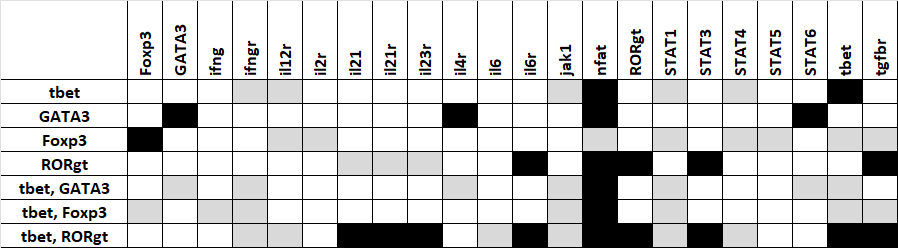
\includegraphics[width=\textwidth]{figs-datamod2023/slicing_results.png}
%	\end{center}
%	\caption{Results of slicing analysis. Black cells identify genes (in columns) that are strictly necessary for the achievement of each target (in rows). Gray cells identify relevant genes. White cells identify genes that are not relevant.}
%	\label{fig:slicing-result}
%\end{figure*}
%
%The table in Figure \ref{fig:slicing-result} allows us to assess necessity, relevance and specificity of each internal gene for each phenotype. In particular, for the four phenotypes characterized by a single transcription factor we can observe that:
%\begin{itemize}
%	\item for target Tbet, the analysis suggests that IFNgR and Jak1 are two relevant genes with high specificity, although they are not strictly necessary for the achievement of the target (i.e., their inhibition or knock-out does not guarantee that the target will not be reached);
%	\item for target GATA3, the analysis suggests that IL4R and STAT6 are strictly necessary and highly specific;
%	\item for target Foxp3, the analysis suggests that IL2R and STAT5 are relevant and highly specific, although not strictly necessary; and
%	\item for target RORgt, the analysis suggests that IL6R and STAT3 are strictly necessary and highly specific, but also IL21, IL21R and IL23 result to be particularly important and specific (as also pointed out in \cite{luckheeram2012cd4+}).
%\end{itemize}
%
%This analysis contributes to the understanding of the behaviour of the model, to correct it in case some mistakes are identified and to use it for identifying drug targets. We discussed the relation with other approaches in the literature.

\subparagraph*{\GROOVE experimentation.}

The capabilities of \GROOVE called upon for this case study are very similar to those in \Cref{sec:cmsb2024}; the main difference lies in the specific interest in attractors. Indeed, in contrast to the situation for comorbidities, here after the initial selection of a profile, the context does not cause any more nondeterminism; hence every profile eventually ends up in such an attractor.

A trace ending in a loop, sometimes called a ``lollipop'', is in fact precisely what LTL properties are checked over; hence an LTL property violation takes the form of a lollipop. This means that we can find attractors with specific properties by formulating their non-existence in LTL, and then finding a counter-example through model checking. For instance, the following formulas deny the reachability of an attractor in which \texttt{tbet} and \texttt{gata3} are expressed:

\begin{itemize}
\item \verb=!G(F gata3 & F tbet)= (separate expression)
\item \verb=!GF (gata3 & tbet)= (simultaneous expression)
\end{itemize}

Using the start graph derived from \BioResolve using the process outlined in \Cref{fig:chain}, both of these formulas yield counterexamples, meaning that \texttt{tbet} and \texttt{gata3} \emph{can} in fact be (recurrently) expressed simultaneously. Using a variation of the process outlined in \Cref{sec:RS2GTS}, we can once more visualise a trace leading to such a recurrent state. The variation lies in the fact that, this time, we do not  want to show the causal history of a \emph{single} forbidden entity, but rather of the combination of two distinct entities. Fortunately, this is just a matter of creating another rule, \gatatbet, which applies precisely when \verb=gata3 & tbet= holds. On this basis we can go through the steps outlined in \Cref{fig:chain}, resulting in the occurrence graph displayed in \Cref{fig:datamod-pruned}.

\begin{figure}\centering
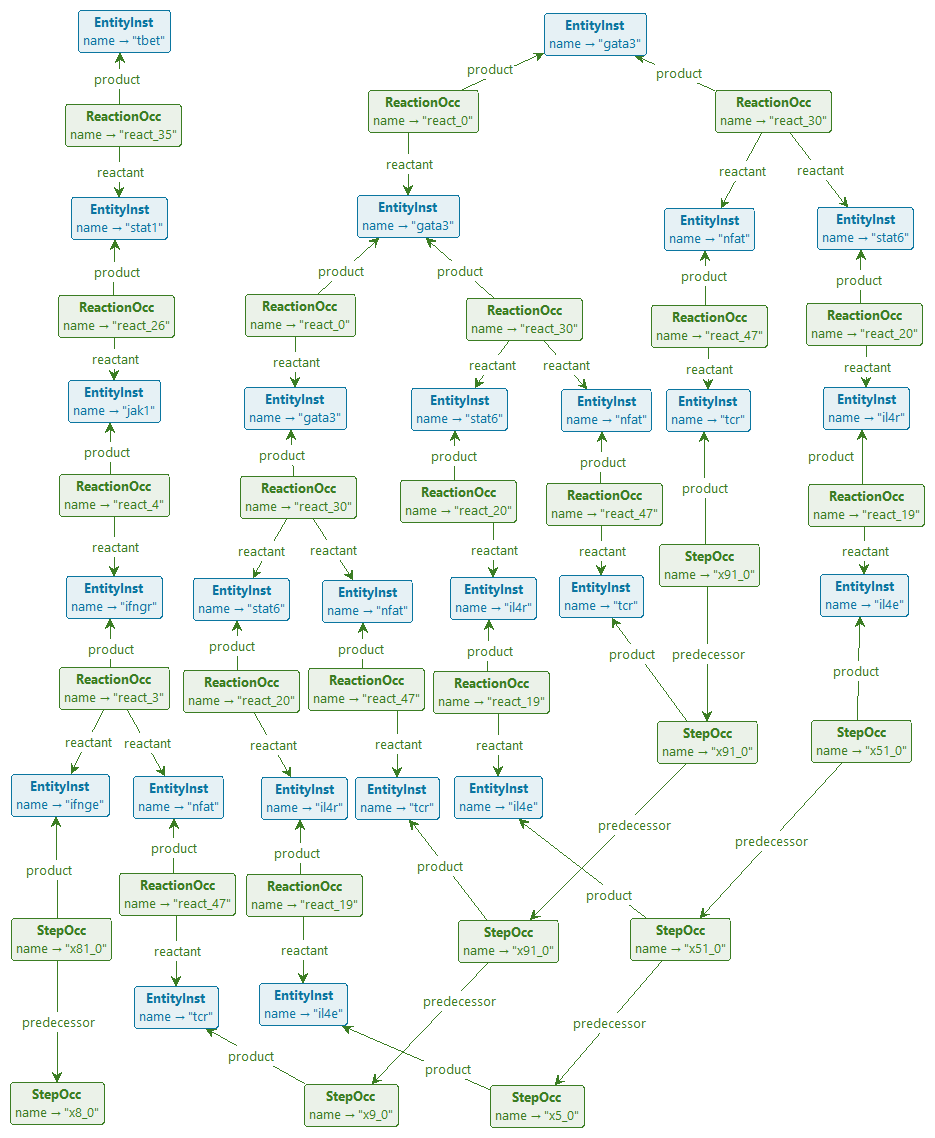
\includegraphics[scale=.25]{figs/datamod-pruned}
\caption{Occurrence graph for the simultaneous expression of \texttt{gata3} and \texttt{tbet}}
\label{fig:datamod-pruned}
\end{figure}

This complements the observation embodied in \cite[Fig.~7]{datamod2023-NaCo} that for the combination of \texttt{tbet} and \texttt{gata3}, the context has to provide the stimuli \texttt{ifnge} (produced here by the \StepOcc named \texttt{x81\_0}), \texttt{tcr} (repeatedly produced by \StepOcc{}s named \texttt{x91\_0}) and \texttt{il4e} (also repeatedly produced, by \StepOcc{}s named \texttt{x51\_0}). In more detail, we see that \texttt{tbet} derives, in a linear sequence of four \ReactionOcc{}s, from \texttt{ifnge} and \texttt{tcr}, whereas \texttt{gata3} derives, in 3 successive combinations of simultaneous \ReactionOcc{}s, from \texttt{tcr} and \texttt{il4e}. Moreover, the genes produced along the way are precisely the ones reported in \cite[Fig.~8(a)]{datamod2023-NaCo}, using the slicing algorithm of that paper, as being relevant for the expression of \texttt{tbet} and \texttt{gata3}.

\medskip\noindent Besides the production of such occurrence graphs for specific cases, \GROOVE can also be used once more to directly confirm the findings of \cite[Figs. 7 and~8]{datamod2023-NaCo}, by expressing them as CTL formulas similar to the one reported in \Cref{fig:table-from-cmsb2024}. In this context, it is relevant to report that, in contrast to \BioResolve, where (as reported above) time and space performance were a bottleneck in the analysis of this model, \GROOVE can fully explore the state space in approximately 3 seconds.

\subparagraph*{Discussion}

Compared to the results in \cite{datamod2023-NaCo}, the advantages of \GROOVE are threefold (reiterating the observations made for the previous two cases):
%
\begin{itemize}
\item LTL model checking allows to express, in a flexible manner, the scenarios one wants to investigate;
\item The occurrence graph visualisation offers analysis possibilities beyond the outcome of the slicing algorithm;
\item The performance of \GROOVE is an order of magnitude better than that of \BioResolve
\end{itemize}


